\subsection{Email Confirmation}

%For the main pages put a mockup and describe it in detail.

%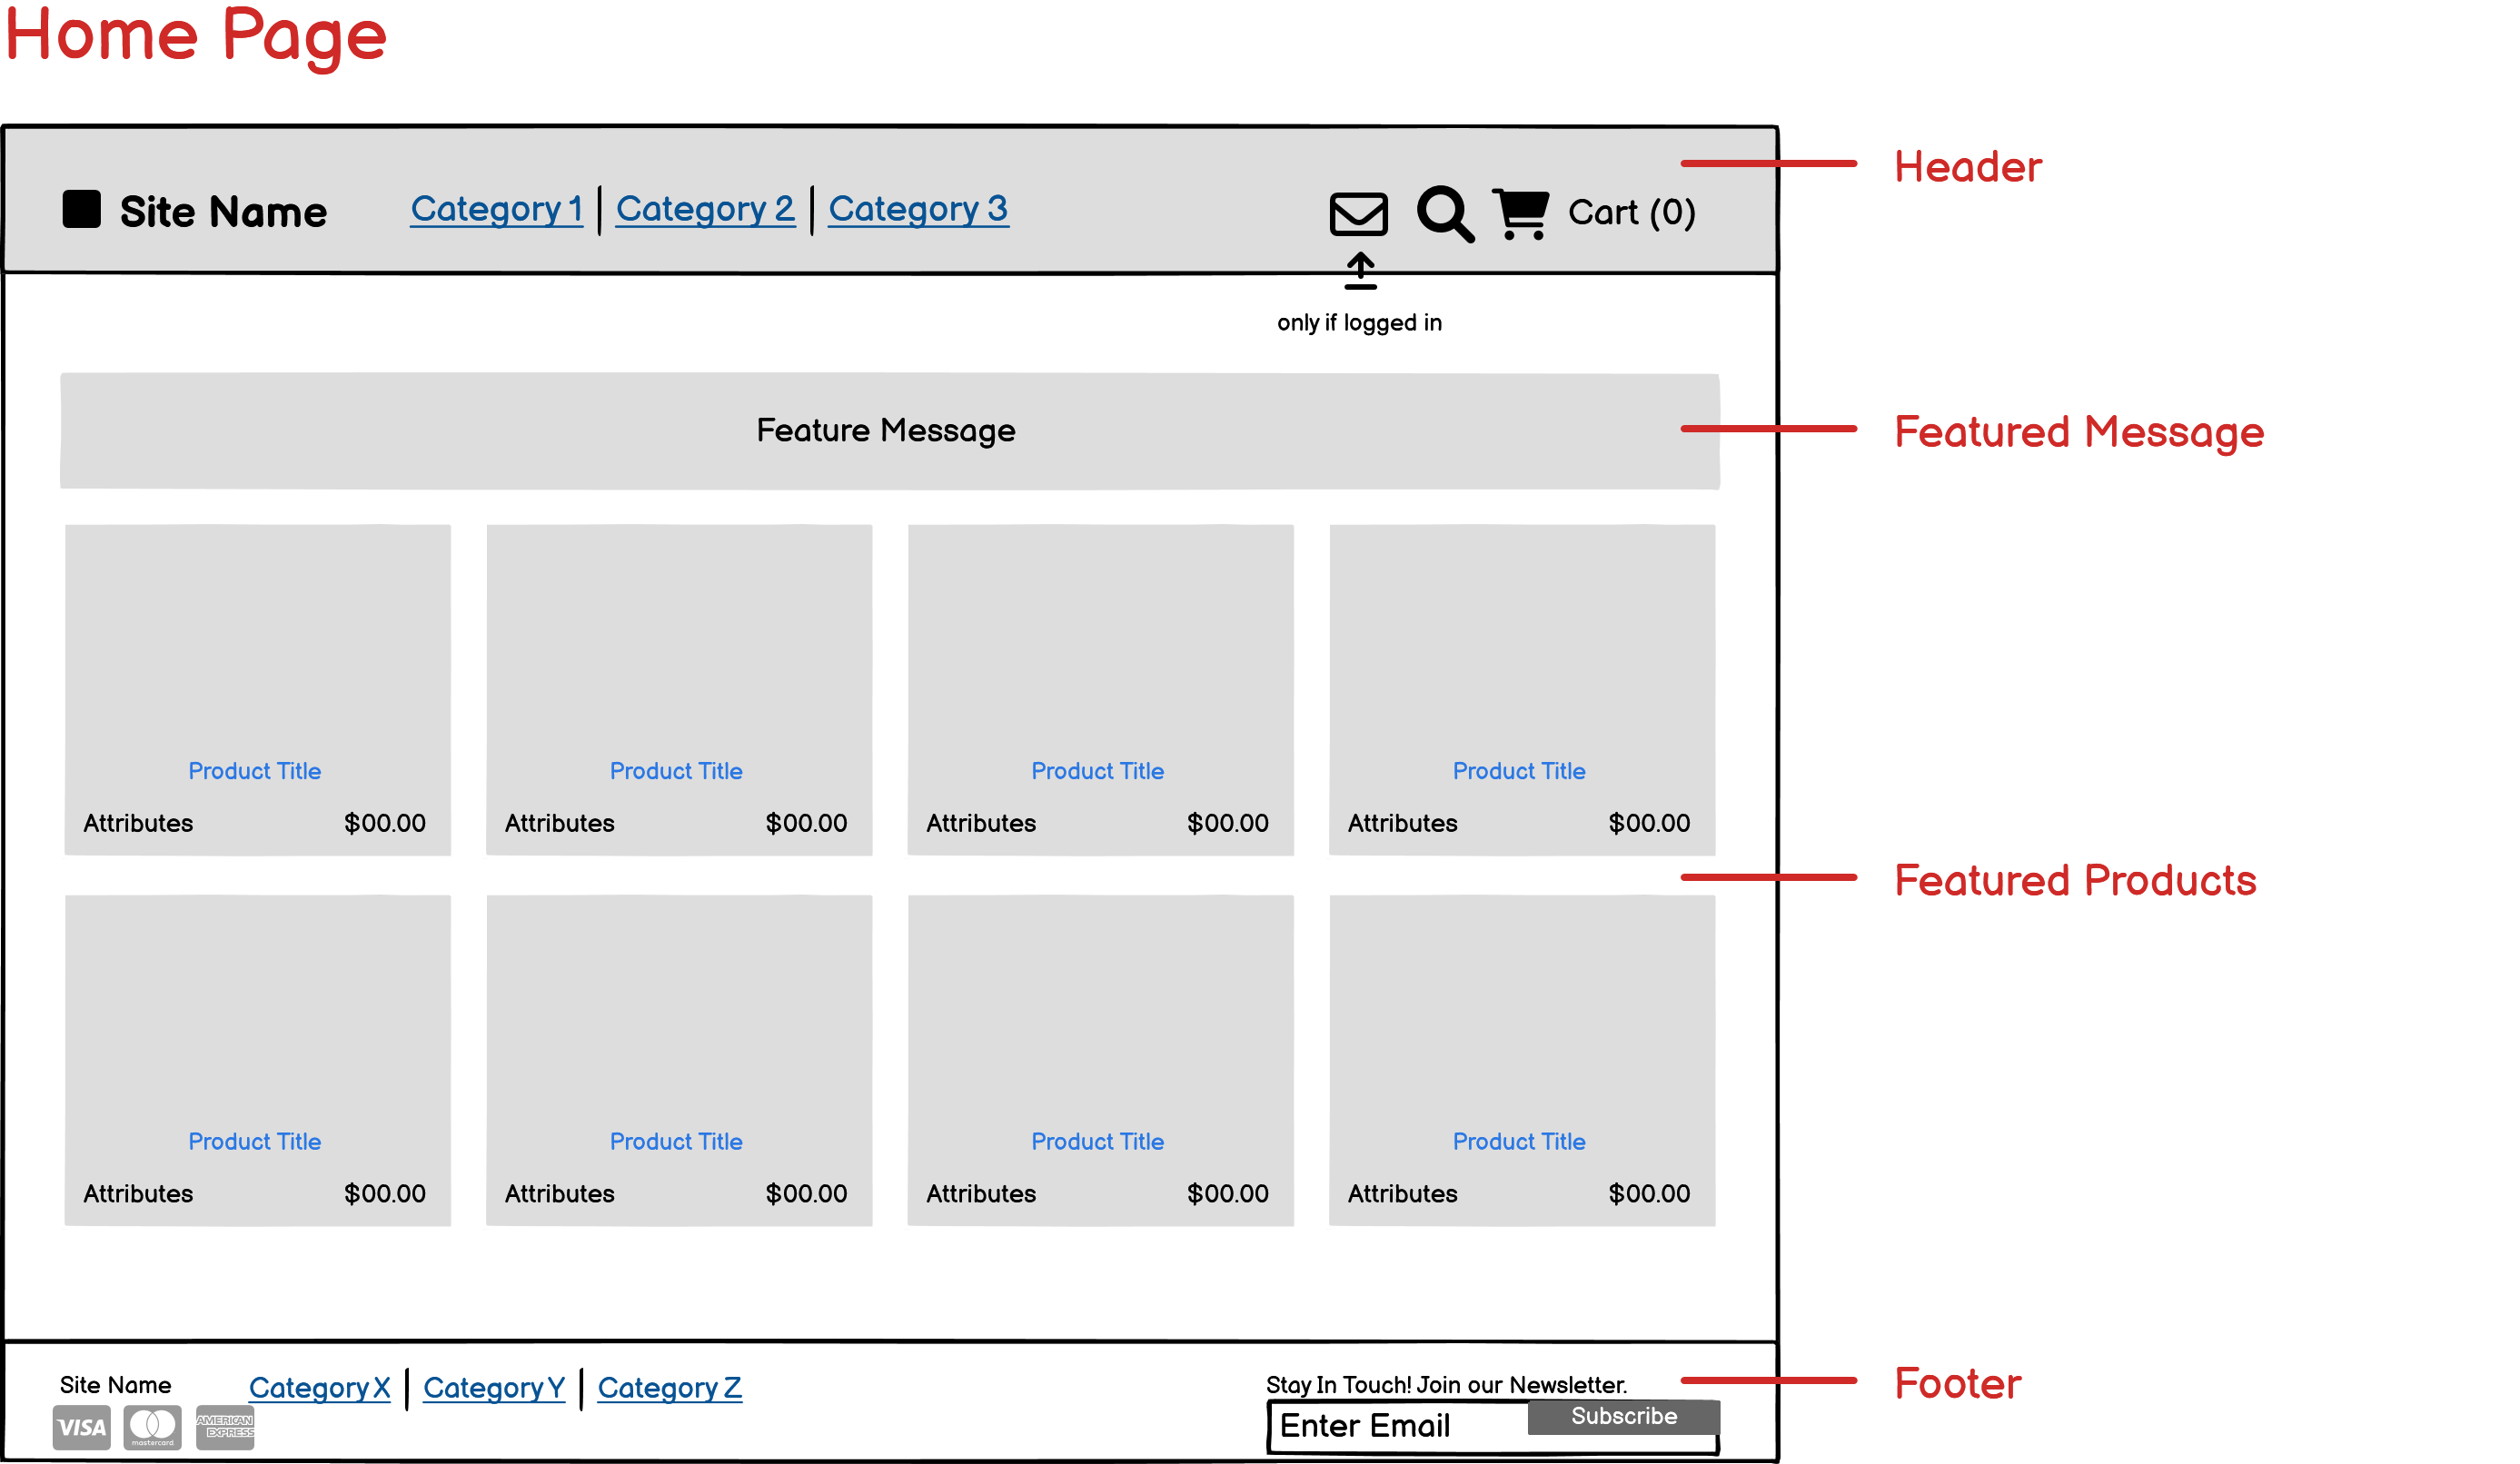
\includegraphics[scale=0.5]{logos/Images/pages/Home Page.png}

\begin{figure}[h]
    \centering
    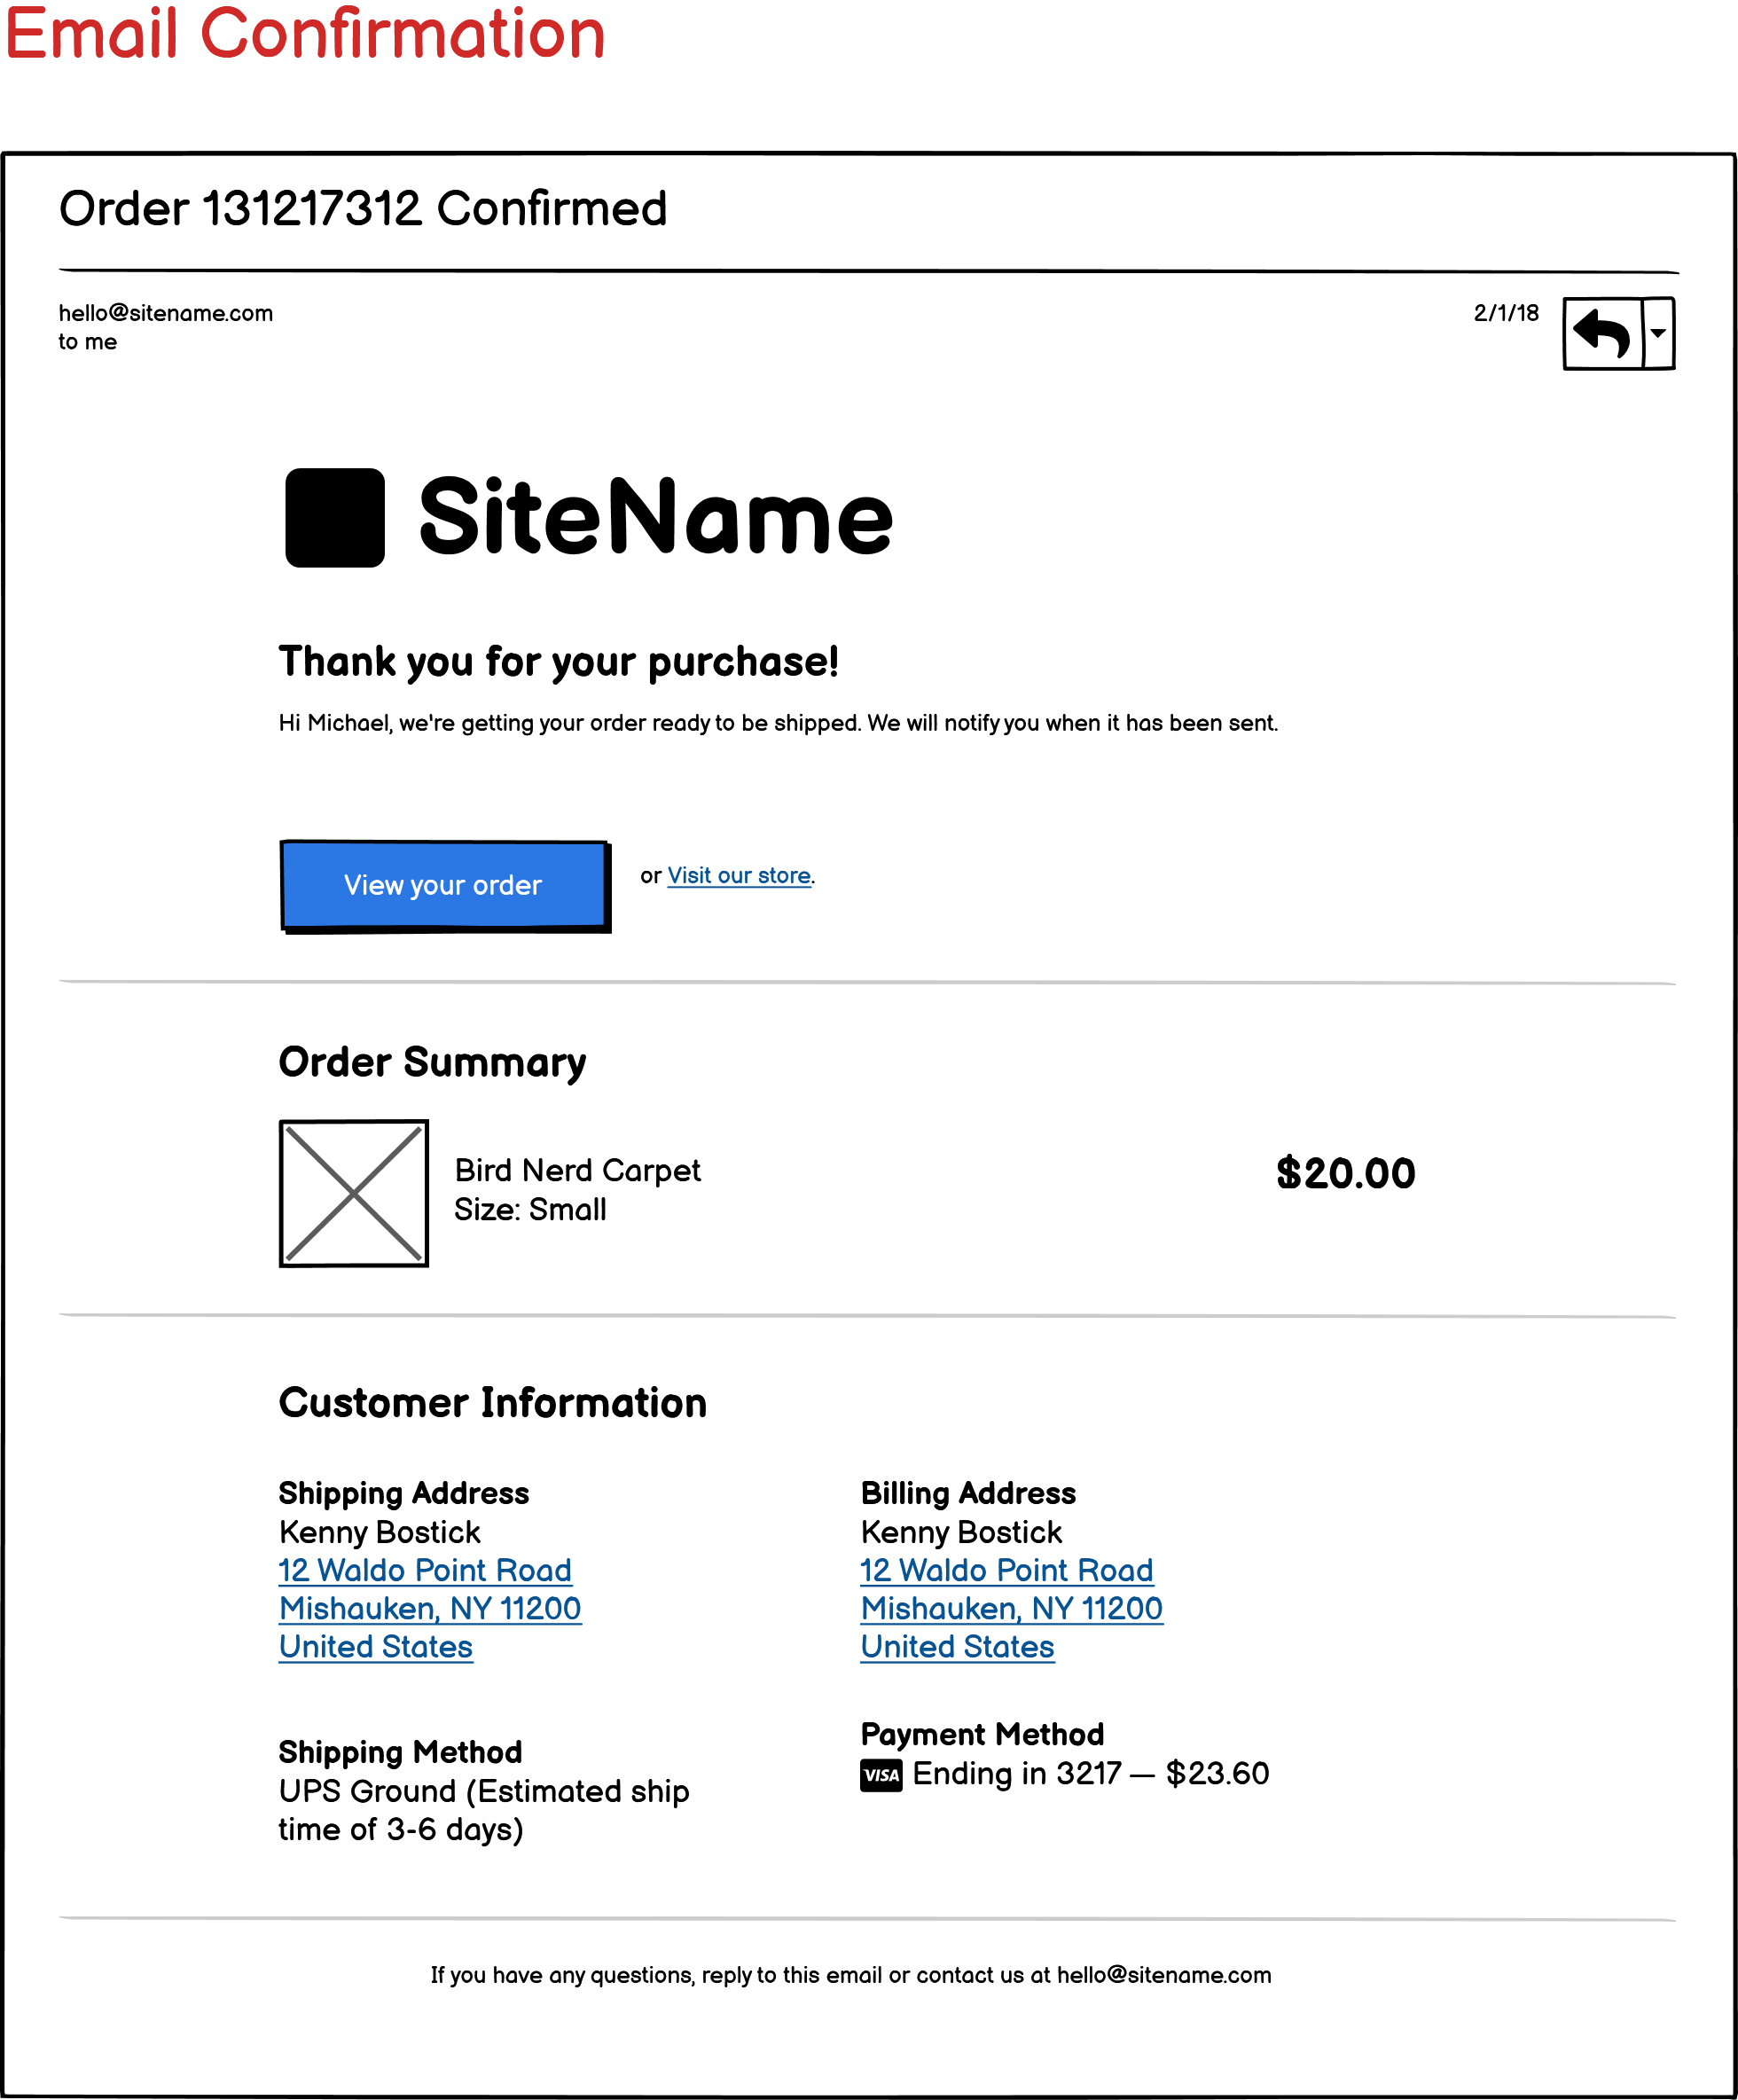
\includegraphics[scale=0.3]{logos/Images/pages/Email Confirmation.png}
    \caption{Email Confirmation}
    \label{fig:my_label}
\end{figure}
\hfill \break
After an order is placed on this website, a confirmation email is sent to the user to confirm the successful completion of the order. The subject and first line of the email will contain the order number to allow the user to easily identify the order.\\\\
The email starts with the website's logo and company name to ensure that the user can verify the authenticity of the email. This is followed by a brief acknowledgement of the order and a button that allows the user to view the details of their order.\\\\
Below this is a summary of the order, including the price and items purchased. This information is intended to give the user a clear overview of the order.\\\\
At the very bottom of the email is the shipping and billing address information, as well as the delivery method and payment method. This information is intended to give the user a clear idea of what to expect and how to track their order.\\\\
Overall, this confirmation email provides the user with a quick and easy way to confirm that their order has been successfully completed. The clear and detailed information ensures that the user is always aware of the status of their order.